\documentclass[conference,a4paper]{IEEEtran}
\pdfminorversion=6
\IEEEoverridecommandlockouts
% The preceding line is only needed to identify funding in the first footnote. If that is unneeded, please comment it out.
% Template version as of 6/27/2024. The a4paper option is kept because the
% IEEE-RIVF 2026 call for papers requires PDF, IEEE standard, A4 size.

\usepackage{cite}
\usepackage{amsmath,amssymb,amsfonts}
\usepackage{algorithmic}
\usepackage{graphicx}
\usepackage{textcomp}
\usepackage{xcolor}
% Required so BibTeX-emitted URLs (with underscores) typeset correctly.
\usepackage{url}
% Vietnamese example phrases in the body require the T5 font encoding.
\usepackage[T5,T1]{fontenc}
\usepackage[utf8]{inputenc}
\newcommand{\viet}[1]{{\fontencoding{T5}\fontfamily{ptm}\selectfont #1}}
\def\BibTeX{{\rm B\kern-.05em{\sc i\kern-.025em b}\kern-.08em
    T\kern-.1667em\lower.7ex\hbox{E}\kern-.125emX}}
\begin{document}

\title{SalePilot: Constraint-First Grounded Decision Support for Vietnamese Retail Consultation}

% TODO: Replace BOTH placeholder blocks below with real author/affiliation data
% before EDAS submission (https://edas.info/N35414). Blind-review policy
% must be confirmed from the CFP before deciding whether to include names.
\author{\IEEEauthorblockN{1\textsuperscript{st} Given Name Surname}
\IEEEauthorblockA{\textit{dept. name of organization (of Aff.)} \\
\textit{name of organization (of Aff.)}\\
City, Country \\
email address or ORCID}
\and
\IEEEauthorblockN{2\textsuperscript{nd} Given Name Surname}
\IEEEauthorblockA{\textit{dept. name of organization (of Aff.)} \\
\textit{name of organization (of Aff.)}\\
City, Country \\
email address or ORCID}
}

\maketitle

\begin{abstract}
Vietnamese retail consultation must preserve requirements across turns and never recommend items that violate budgets or physical limits. SalePilot grounds this task in fail-closed constraint filtering with verifiable decision evidence.

The system separates a deterministic constraint-first recommender from optional large language model (LLM) orchestration. Each recommendation carries constraint states, admission counts, provenance, and a catalog hash for rechecking.

We characterize a crawled dataset of 13{,}754 products across 119 categories and 436 brands from a major Vietnamese electronics retailer, together with 10 anonymized purchase-completion conversations containing 56 tool-call invocations across 7 distinct tools. We evaluate on a sealed benchmark of 40 Vietnamese episodes over a hash-pinned catalog snapshot.

Explicit constraint filtering removes every observed violation: 0 in 99 product--constraint checks for both constraint conditions versus 10 in 117 for the price-popularity baseline. The paired bootstrap difference of 0.0855 excludes zero.

All conditions share one parser; category accuracy and slot micro-F1 are identical across conditions. Action accuracy is 0.925 for the price-popularity baseline and 0.850 for both constraint conditions. Ranking differences need relevance labels, scoped to future work. Deployment claims stay prototype-scoped. Artifacts are hash-chained.
\end{abstract}

\begin{IEEEkeywords}
conversational recommender systems, decision support, Vietnamese language, constraint satisfaction, explainable recommendation, reproducibility
\end{IEEEkeywords}

\section{Introduction}
Conversational recommender systems (CRSs) turn one-shot ranking into an interaction that can elicit preferences, explain options, and react to feedback~\cite{jannach2021survey}.

For appliances and electronics, a short request may omit budget, room or household size, physical limits, or energy preferences. The system must decide whether to clarify, recommend, answer a policy question, or abstain.

Selective questioning has been formalized for recommendation~\cite{christakopoulou2016towards}. Estimation--action--reflection separates preference estimation, action choice, and feedback handling~\cite{lei2020ear}.

Recent work uses LLMs as planners over recommender tools~\cite{huang2025interecagent}. Hybrid multi-agent designs have also been studied for e-commerce consultation~\cite{nie2024hybrid}.

Fluency alone is insufficient. CRS evaluation must distinguish component quality from user experience~\cite{jannach2023evaluating}. Agent benchmarks likewise motivate multi-turn tests in executable environments~\cite{liu2024agentbench}.

SalePilot asks three questions. Does explicit filtering reduce observed hard-constraint violations? Does its hybrid ranker outperform a lexical-filter baseline? Which system and deployment claims do the current artifacts support?

The paper makes four contributions:

\begin{enumerate}
\item A Vietnamese prototype that combines structured need accumulation, deterministic ranking, optional LLM orchestration, and a multi-backend catalog;

\item A characterization of a real Vietnamese retail dataset---13{,}754 products, 119 categories, 1{,}348 spec attribute types, and 10 annotated purchase conversations---that quantifies category imbalance, price skew, field coverage gaps, and tool-call patterns;

\item A versioned evidence dictionary for deterministic recommendations, including selected product facts, computed constraint states, fail-closed admission counts, and catalog identity metadata;

\item A sealed, manifest-linked evaluation of three deterministic conditions on one catalog snapshot, with paired bootstrap inference, explicit custody, and evidence limits.
\end{enumerate}

The experiment does not test the Lead loop, specialist roles, response fluency, interface quality, conversion, or field effectiveness. These boundaries prevent component-level results from becoming system-wide claims.

\section{Related Work and Positioning}
\subsection{CRS background and tool-grounded agents}
CRS research spans intent handling, knowledge, interaction, and evaluation~\cite{jannach2021survey}. The System Ask--User Respond paradigm explicitly elicits attributes~\cite{zhang2018systemask}. EAR separates preference estimation, asking or recommending, and reflection after feedback~\cite{lei2020ear}. SalePilot adopts this decomposition as inspectable rules and state, not as a reproduction of either learned model.

ReAct interleaves model reasoning with actions and observations~\cite{yao2023react}. Multi-agent work organizes systems through profiles, communication, and skills~\cite{guo2024multiagents}. AutoGen provides a programmable precedent for multi-agent conversation~\cite{wu2024autogen}. External stores motivate retrieval-augmented generation~\cite{lewis2020rag} and retrieval-in-the-loop conversation~\cite{shuster2021retrieval}. SalePilot retrieves catalog records but keeps product recommendation on a deterministic path when a request is sufficiently clear.

\subsection{Evaluation and reproducibility}
Explainable recommendation serves different stakeholders and goals~\cite{zhang2020explainable}. Simple baselines can expose weak progress claims~\cite{ferraridacrema2021troubling}. Offline protocols can also contain methodological flaws~\cite{hidasi2023widespread}. We therefore separate action, extraction, constraint, and deployment evidence.

\section{SalePilot Design}
\subsection{System boundary and orchestration}
Fig.~\ref{fig1} shows the boundary: a runtime path from channels to ranking, and the deterministic decision data that every emitted recommendation carries.

\begin{figure*}[!t]
\centerline{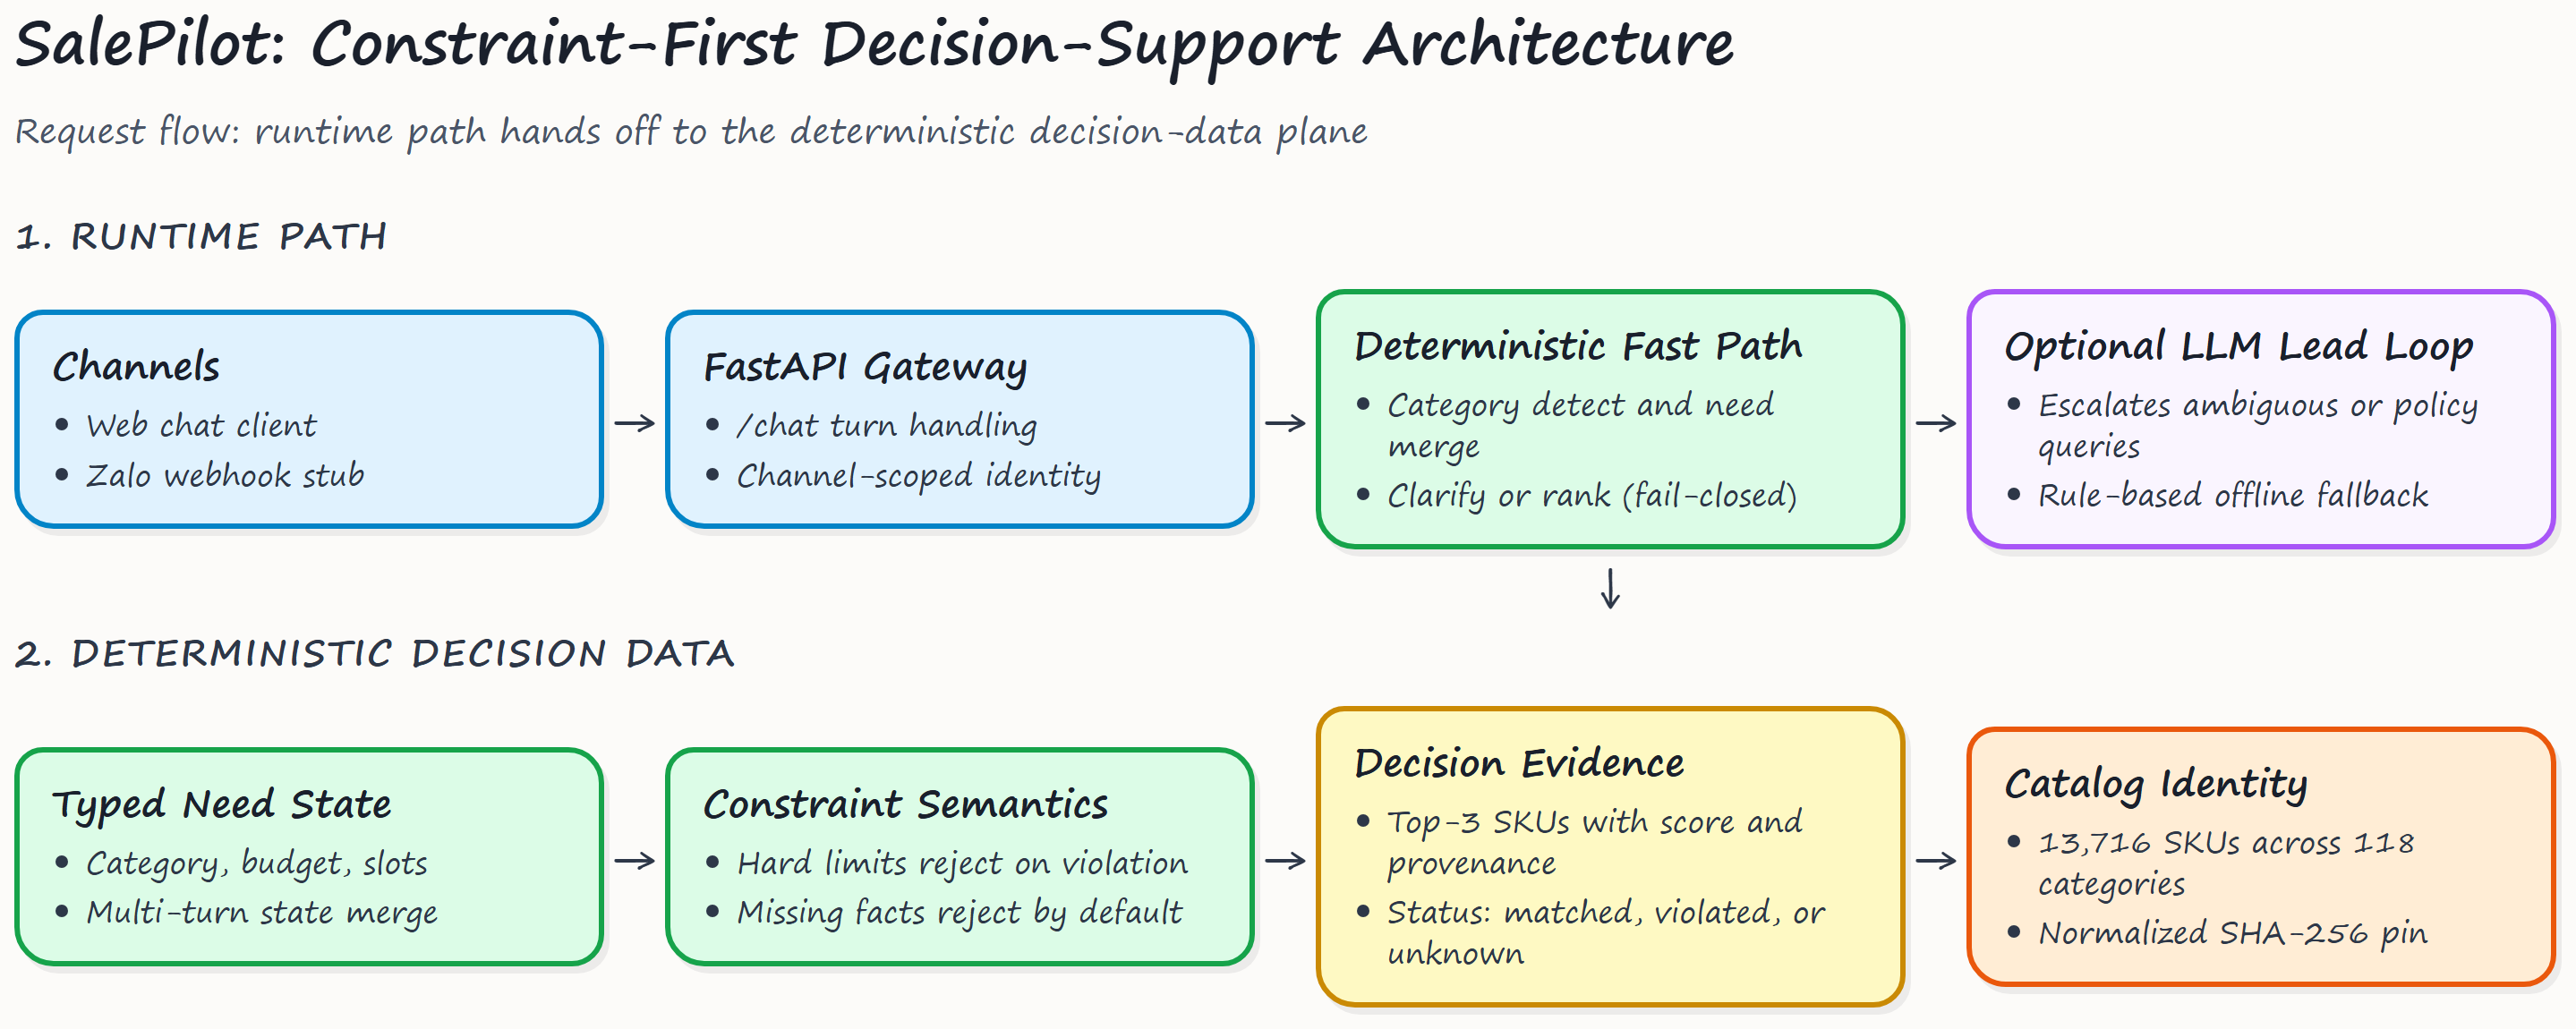
\includegraphics[width=\textwidth]{figures/system_architecture_v2.png}}
\caption{SalePilot architecture. The runtime path (top) separates the deterministic fast path from the optional LLM Lead loop; the decision data plane (bottom) turns typed need state and fail-closed constraint semantics into evidence tied to a hash-pinned catalog identity.}
\label{fig1}
\end{figure*}

Clear product requests enter a deterministic fast path for category detection, need merge, clarification, and ranking. With no LLM key, a rule-based coordinator also handles comparison, FAQ, CRM, and escalation branches.

With an LLM key, the same fast path is attempted first. Ambiguous requests may enter a Lead--tool loop. Catalog and knowledge are direct Lead tools; short tool-scoped loops exist for named specialist roles.

Fig.~\ref{fig_request} shows the three-stage nominal workflow: ingress and routing, decision pathways (deterministic typed-need route versus LLM orchestrator), and assembly with evidence export and channel delivery.

\begin{figure}[!t]
\centerline{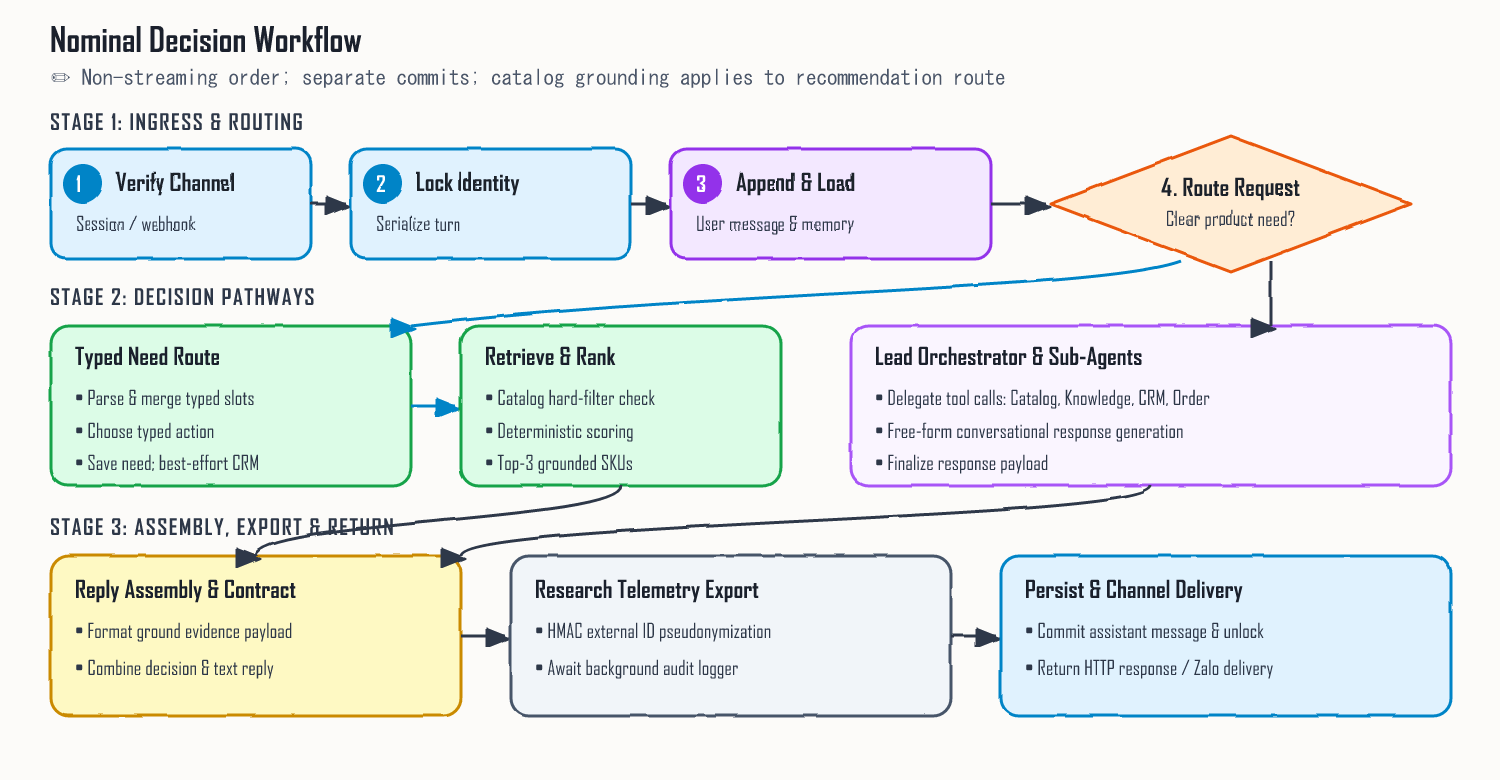
\includegraphics[width=\columnwidth]{figures/request_workflow.png}}
\caption{Nominal decision workflow. Stage~1 routes by channel and identity; Stage~2 branches into a deterministic typed-need path or the LLM orchestrator; Stage~3 assembles evidence and delivers the response.}
\label{fig_request}
\end{figure}

The evaluated crawl registry has hand-authored rules for eight core families. Other categories loaded from the catalog receive generic objects with aliases and budget-oriented ranking, but no category-specific need slots.

A separate workbook profile declares 14 categories for that data configuration. The sealed experiment instead uses the crawl profile and a 118-category DMX snapshot.

\subsection{Need state and action policy}
Let $H_t=(u_1,\ldots,u_t)$ be the conversation and $n_t$ a structured need dictionary. A category-aware extractor $E$ and merge operator $M$ update the state:

\begin{equation}
 n_t=M(n_{t-1},E(u_t,c_{t-1})).\label{eq1}
\end{equation}

Fresh nonempty values overwrite matching fields. Priorities are unioned within one category. A category switch drops earlier category fields but retains the old budget when the new turn gives none.

On the keyed fast path, a bare number or recognized room label may fill the first pending slot. The offline coordinator does not apply this resolver, so the two runtime paths are not behaviorally identical.

Runtime routing uses flags rather than a typed action enum. The benchmark allows \texttt{recommend}, \texttt{clarify}, \texttt{compare}, \texttt{faq}, and \texttt{abstain}; the current adapter emits all except \texttt{compare}.

A missing budget triggers clarification unless flexibility is explicit. A core category can also require one primary slot. Generic categories usually require only category and budget before ranking.

Fig.~\ref{figclarify} contrasts a one-shot reply with this clarify-then-recommend policy; the questions shown are a clarification exchange recorded from the running prototype.

\begin{figure}[!t]
\centerline{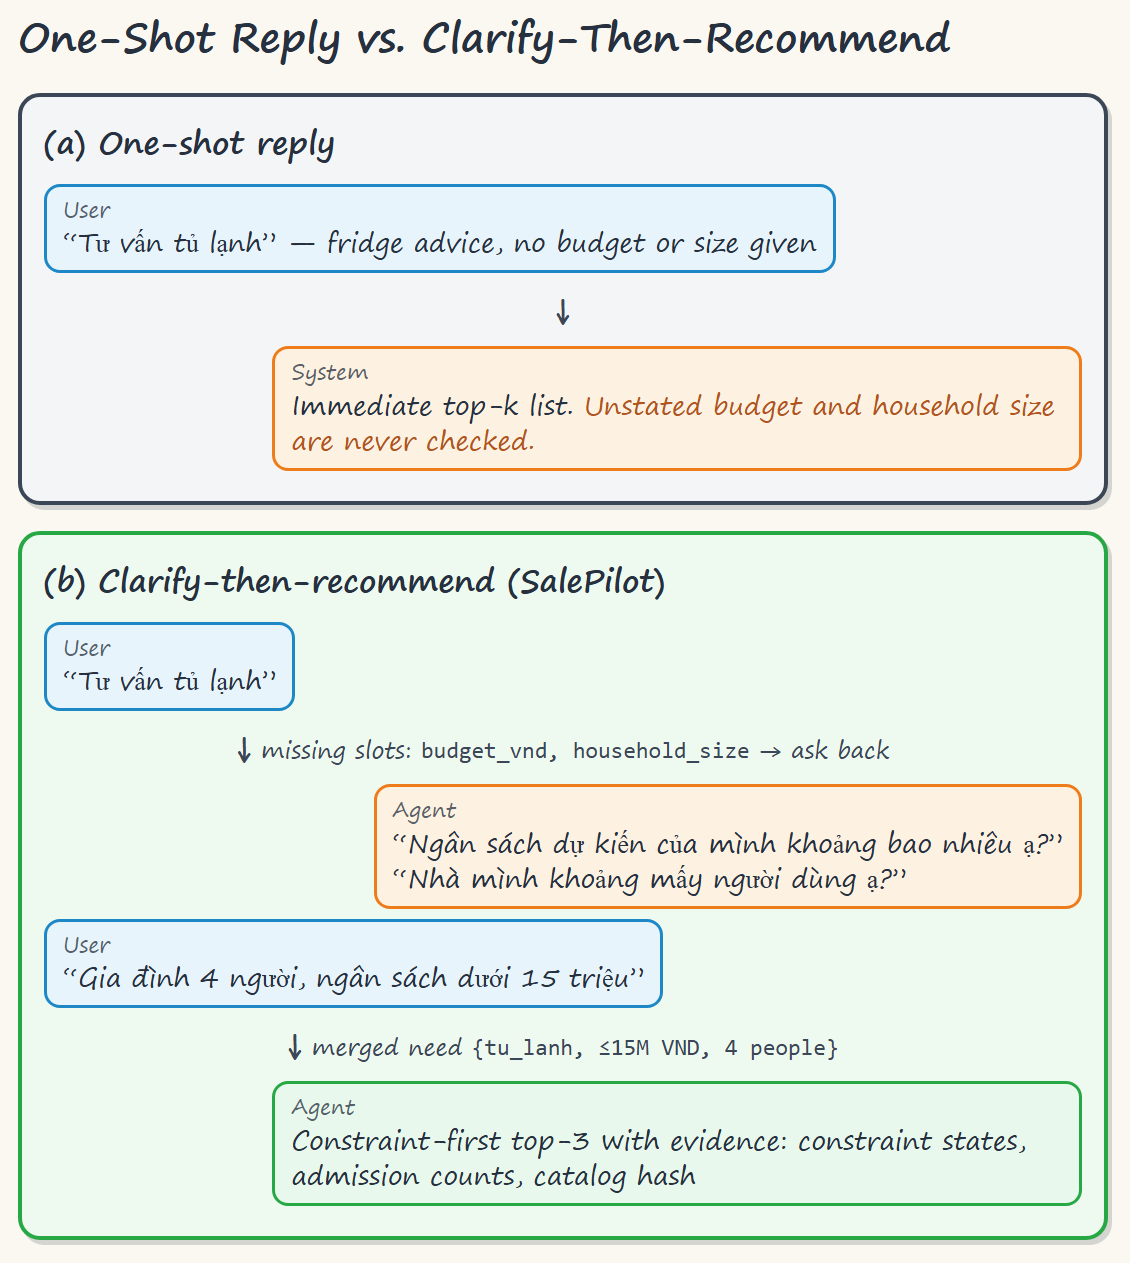
\includegraphics[width=0.85\columnwidth]{figures/clarify_loop.png}}
\caption{One-shot reply versus clarify-then-recommend. With required slots missing, the agent asks back and merges the answers into the need state before constraint-first ranking; the dialogue is recorded from the prototype.}
\label{figclarify}
\end{figure}

In sealed episode test-001, \emph{\viet{Gia đình 3 người cần tủ lạnh dưới 12 triệu inverter}} parses into the category, a household size, a budget, and an energy-saving priority in the recorded need.

\subsection{Constraint-first ranking}
The ranker considers only products with a current price in the selected category. A nonflexible over-budget item is rejected; a flexible over-budget item is retained with a penalty.

Configured range, minimum, maximum, and proximity terms compare normalized product facts with the need. Missing hard facts reject an item unless the slot policy explicitly permits unknown values.

At a high level, the score groups budget, slot, preference, and secondary terms:

\begin{equation}
 S(p,n_t)=B(p,n_t)+\sum_k w_kF_k(p,n_t)+P(p,n_t)+\epsilon(p).\label{eq2}
\end{equation}

The implementation also uses brand, style, rating, popularity, discount, and gift signals. Equation~\eqref{eq2} is a grouping of code paths, not a claim that the evidence payload exposes every addend.

Products are ordered by descending score and ascending price. Equal ties inherit repository order, so repeatability depends on fixed input order rather than a complete cross-backend tie key.

A second pass removes exact model-code duplicates. It favors distinct brands among the first two selections, then fills up to three products. It does not perform similarity-based near-duplicate detection.

Fig.~\ref{fig_ranking} illustrates the four-stage pipeline: the customer need state feeds fail-closed filtering, then stable scoring selects and ranks the top~3, producing an audit payload with catalog hash.

\begin{figure}[!t]
\centerline{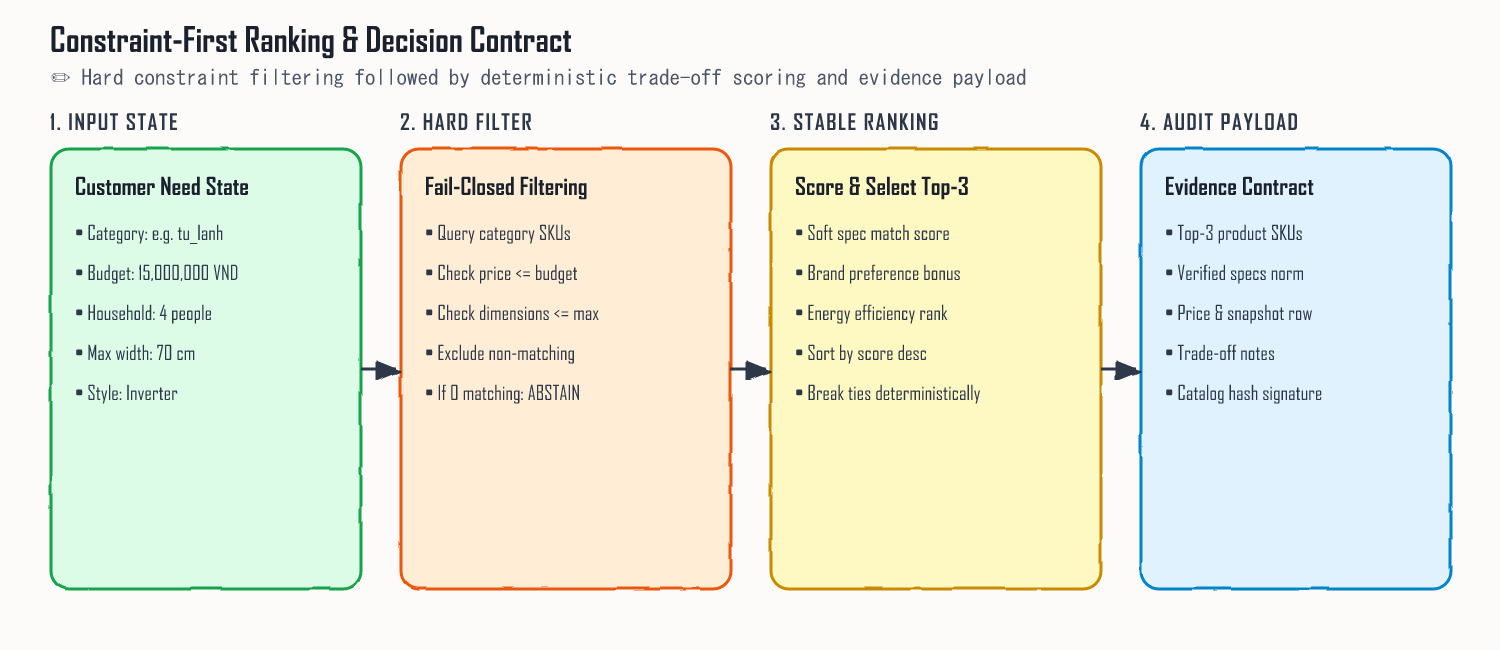
\includegraphics[width=\columnwidth]{figures/ranking_decision_workflow.png}}
\caption{Constraint-first ranking pipeline. Hard constraints reject non-matching products before scoring; the evidence contract ties each recommendation to its catalog identity.}
\label{fig_ranking}
\end{figure}

\subsection{Decision evidence and catalog identity}
Deterministic recommendation routes emit a versioned evidence dictionary containing the parsed need, selected SKUs, match scores, computed constraint statuses, selected product facts, and source metadata.

Constraint states are \texttt{matched}, \texttt{violated}, or \texttt{unknown}. The dictionary counts priced candidates evaluated and those rejected fail-closed. The payload supports rechecking but is not a faithful explanation of LLM reasoning or a complete score reconstruction.

Multiple storage backends (PostgreSQL, MongoDB, JSON snapshot) converge on the same normalized schema. Research scripts pin snapshot bytes; runtime loading computes a semantic digest over the documents that actually load.

\subsection{Operational scope}
The prototype keys state by channel and external identity with an unsigned local UUID. Runtime trajectory capture stores raw content when enabled; the research release forbids raw trajectories and real contact details~\cite{nist2020privacy}. Tool safety controls reduce exposure from command and fetch tools but are not a secure jail~\cite{greshake2023indirect}. Each request is tagged with its serving route for deployment monitoring.

\section{Dataset Analysis}
This section characterizes the DMX dataset to establish the data complexity that SalePilot must handle. Statistics were computed programmatically from the normalized catalog snapshot and anonymized chat trajectories.

\subsection{Product catalog profile}
Table~\ref{tab_dataset} summarizes the catalog. The 13{,}754 products span 119 categories and 436 brands, with prices ranging from 10{,}000 to 380{,}000{,}000~VND (median 1.39M, mean 6.14M). The normalizer extracts 1{,}348 unique specification attribute types from heterogeneous crawled data.

\begin{table}[htbp]
\caption{DMX Catalog Dataset Summary}
\begin{center}
\footnotesize
\begin{tabular}{|l|r|}
\hline
\textbf{Dimension} & \textbf{Value} \\
\hline
Products & 13{,}754 \\
Categories & 119 \\
Brands & 436 \\
Unique spec attribute types & 1{,}348 \\
Price range (VND) & 10K--380M \\
Median / Mean price (VND) & 1.39M / 6.14M \\
Fields with ${>}90\%$ coverage & 10 / 29 \\
Fields with ${<}50\%$ coverage & 4 / 29 \\
\hline
\end{tabular}
\label{tab_dataset}
\end{center}
\end{table}

Fig.~\ref{fig_dataset} shows three distributional views. Panel~(a) reveals severe category imbalance: fashion watches alone account for 22.8\% of products (3{,}138), while core appliance categories such as refrigerators~(251) and air conditioners~(228) comprise under 2\% each. Beyond the top~15 named categories, 104 long-tail categories collectively hold 4{,}566 products (33.2\%), underscoring the need for generic category handling. Panel~(b) shows a log-normal price distribution spanning four orders of magnitude. Panel~(c) shows that 10 fields exceed 90\% coverage, but \texttt{outstanding}~(36\%), \texttt{description}~(17\%), and \texttt{accessories}~(8\%) are sparse---the recommender must handle missing values gracefully.

\begin{figure}[!t]
\centerline{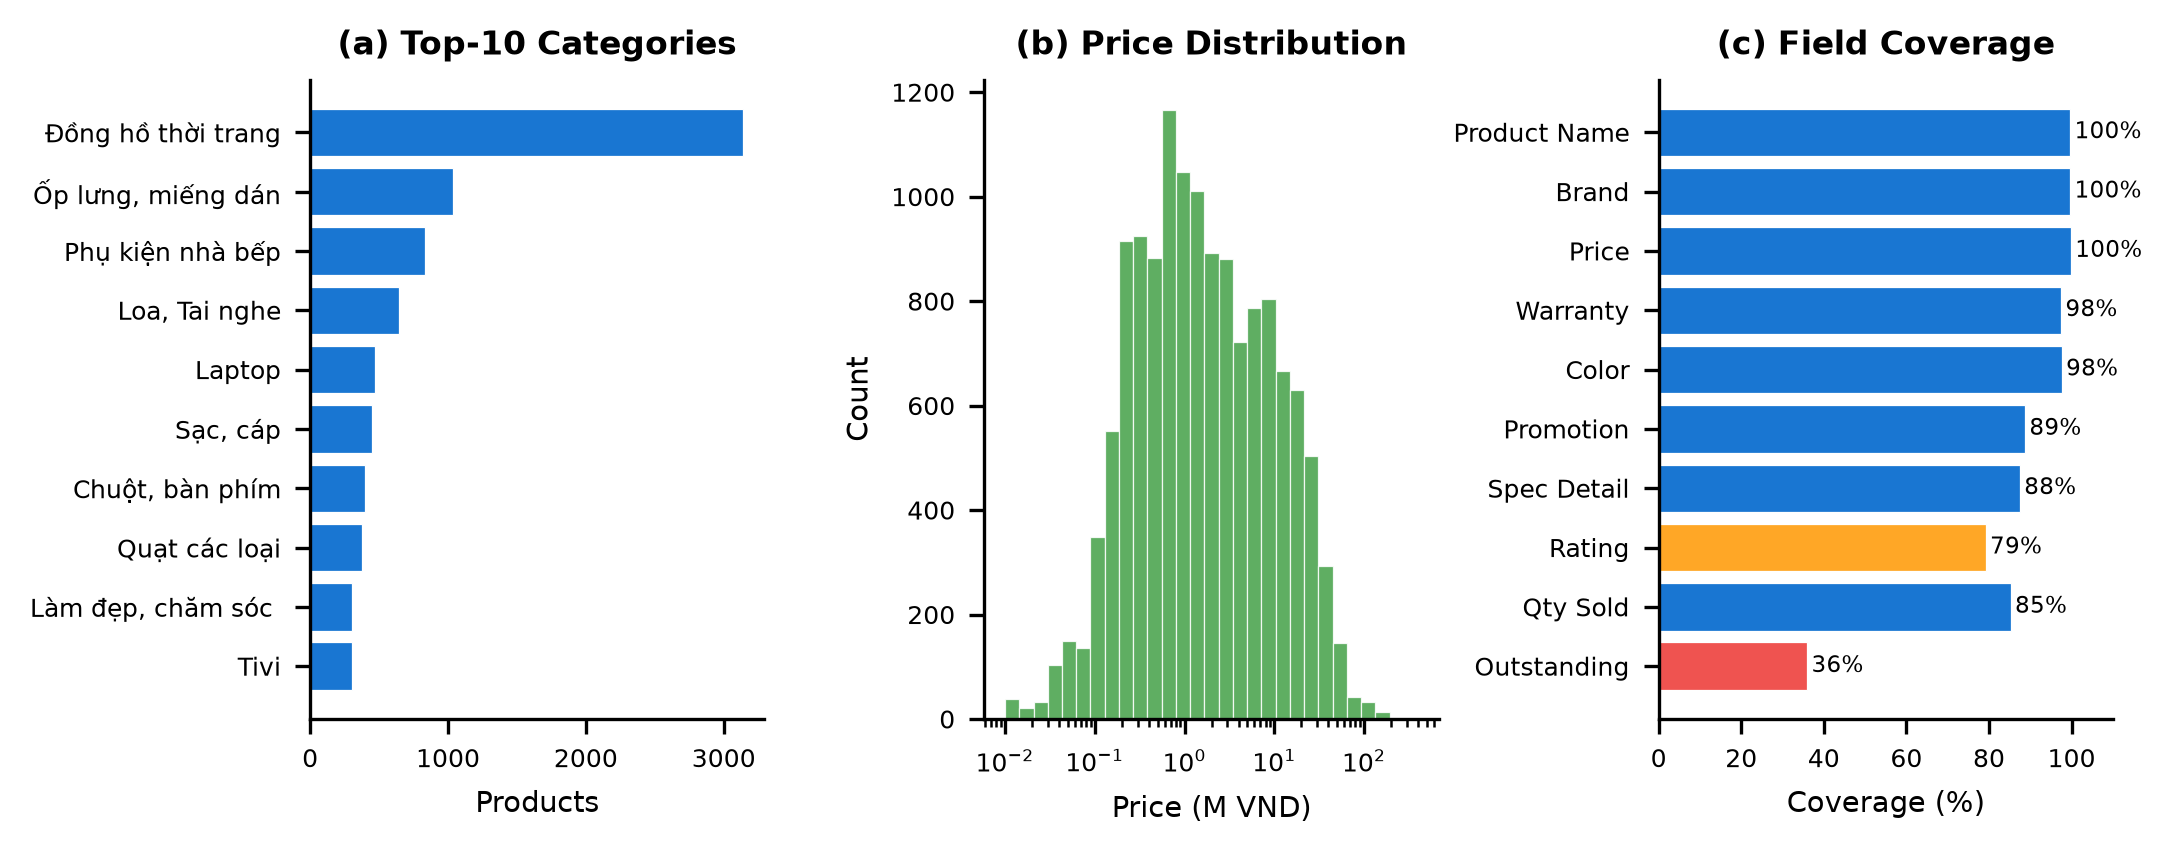
\includegraphics[width=\columnwidth]{figures/dataset_overview.png}}
\caption{DMX dataset overview. (a)~Top-10 categories by product count; (b)~price distribution on log scale; (c)~field coverage percentage with color-coded thresholds.}
\label{fig_dataset}
\end{figure}

Fig.~\ref{fig_catdist} shows the full per-category breakdown. The 15 largest named categories are plotted individually; the remaining 104 are grouped as ``Others'' (4{,}566 products, 33.2\%). This long tail motivates the generic-category fallback path in the recommender.

\begin{figure}[!t]
\centerline{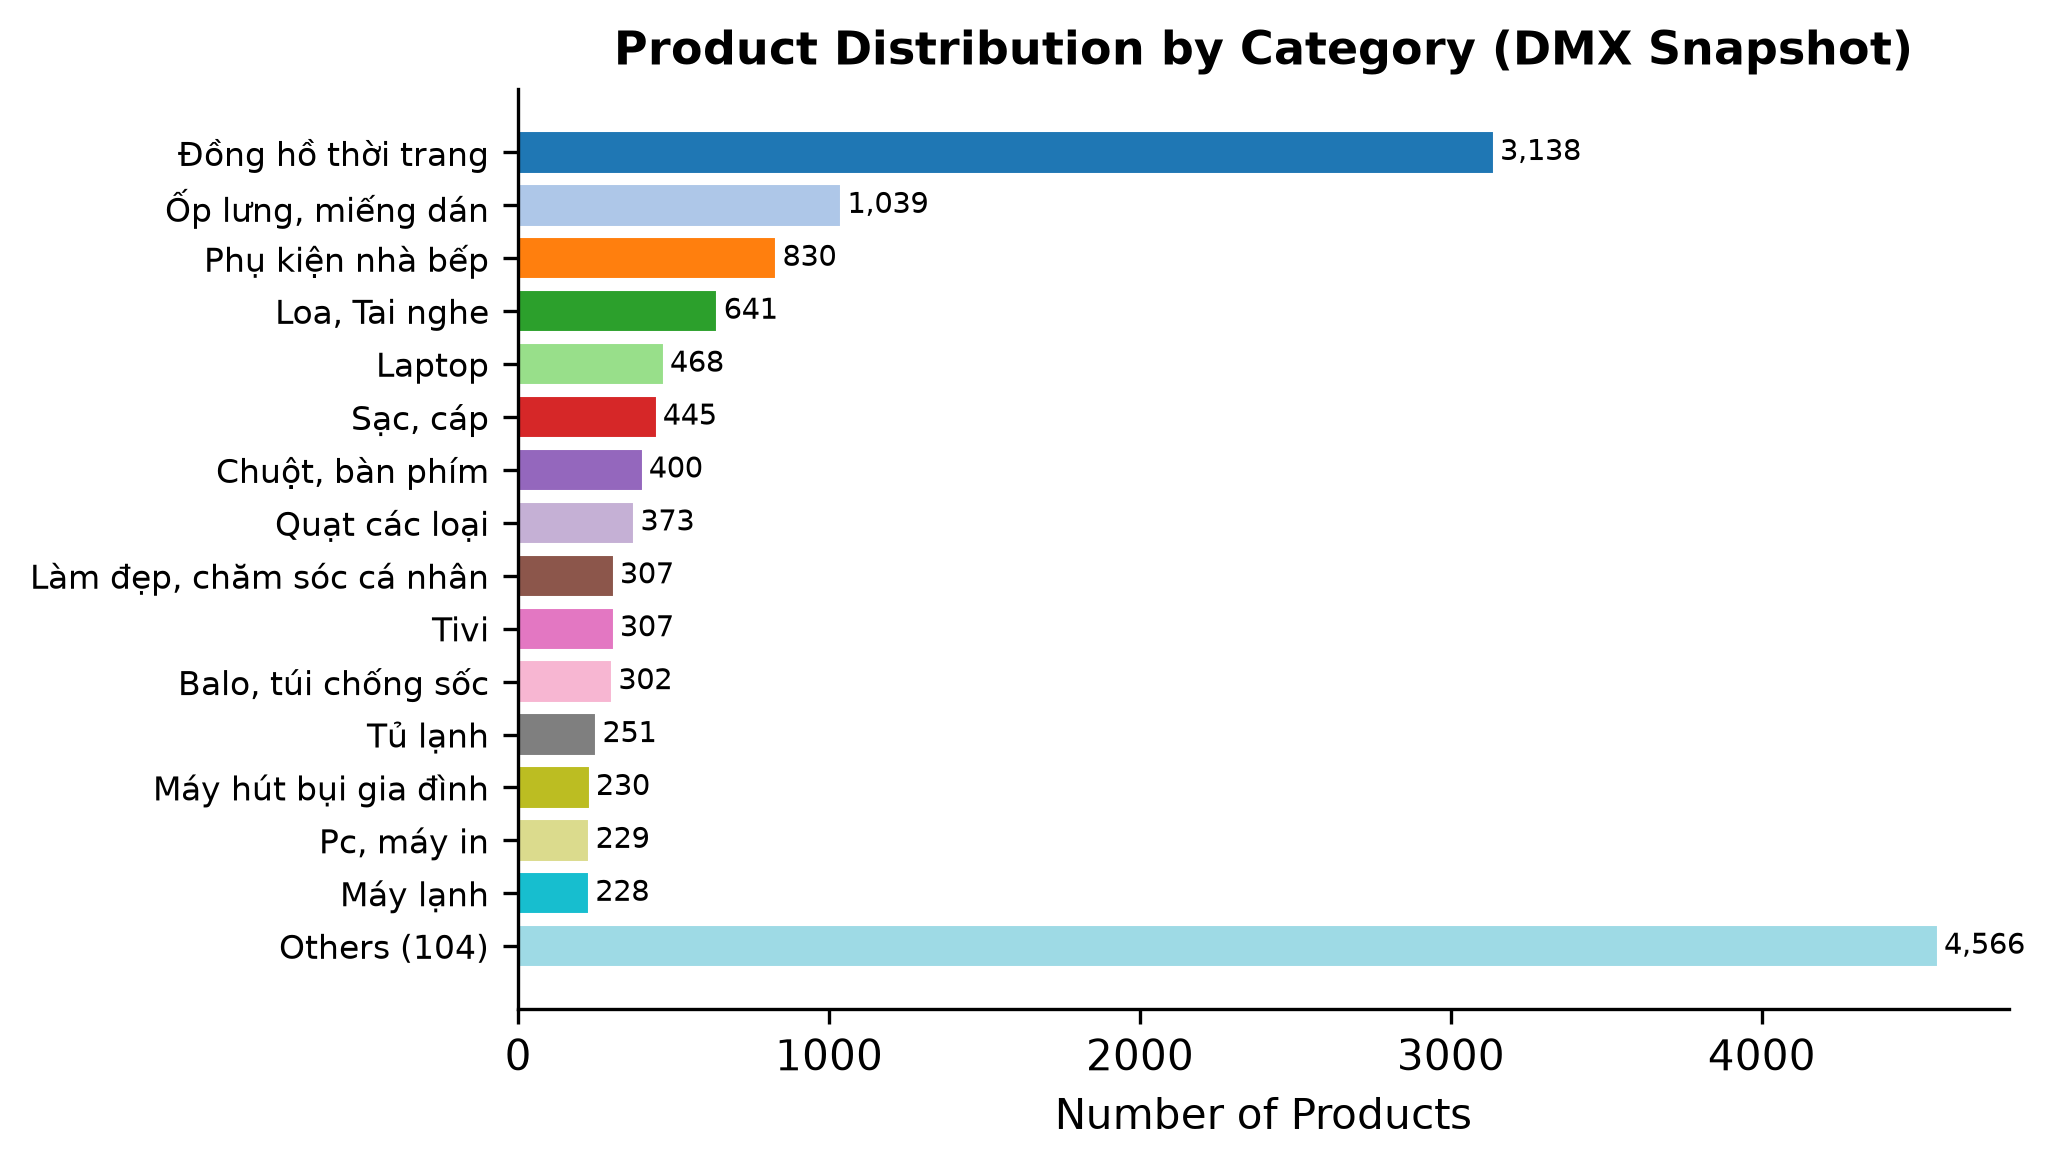
\includegraphics[width=\columnwidth]{figures/dataset_category_distribution.png}}
\caption{Full product distribution across 119 categories. The top~15 named categories are plotted individually; 104 long-tail categories are grouped as ``Others.''}
\label{fig_catdist}
\end{figure}

Fig.~\ref{fig_pricedist} provides a detailed price analysis. The log-scale histogram confirms the right-skewed distribution, while the price-tier pie chart shows that 57\% of products fall in the 500K--10M~VND range, with only 1.3\% exceeding 50M~VND.

\begin{figure}[!t]
\centerline{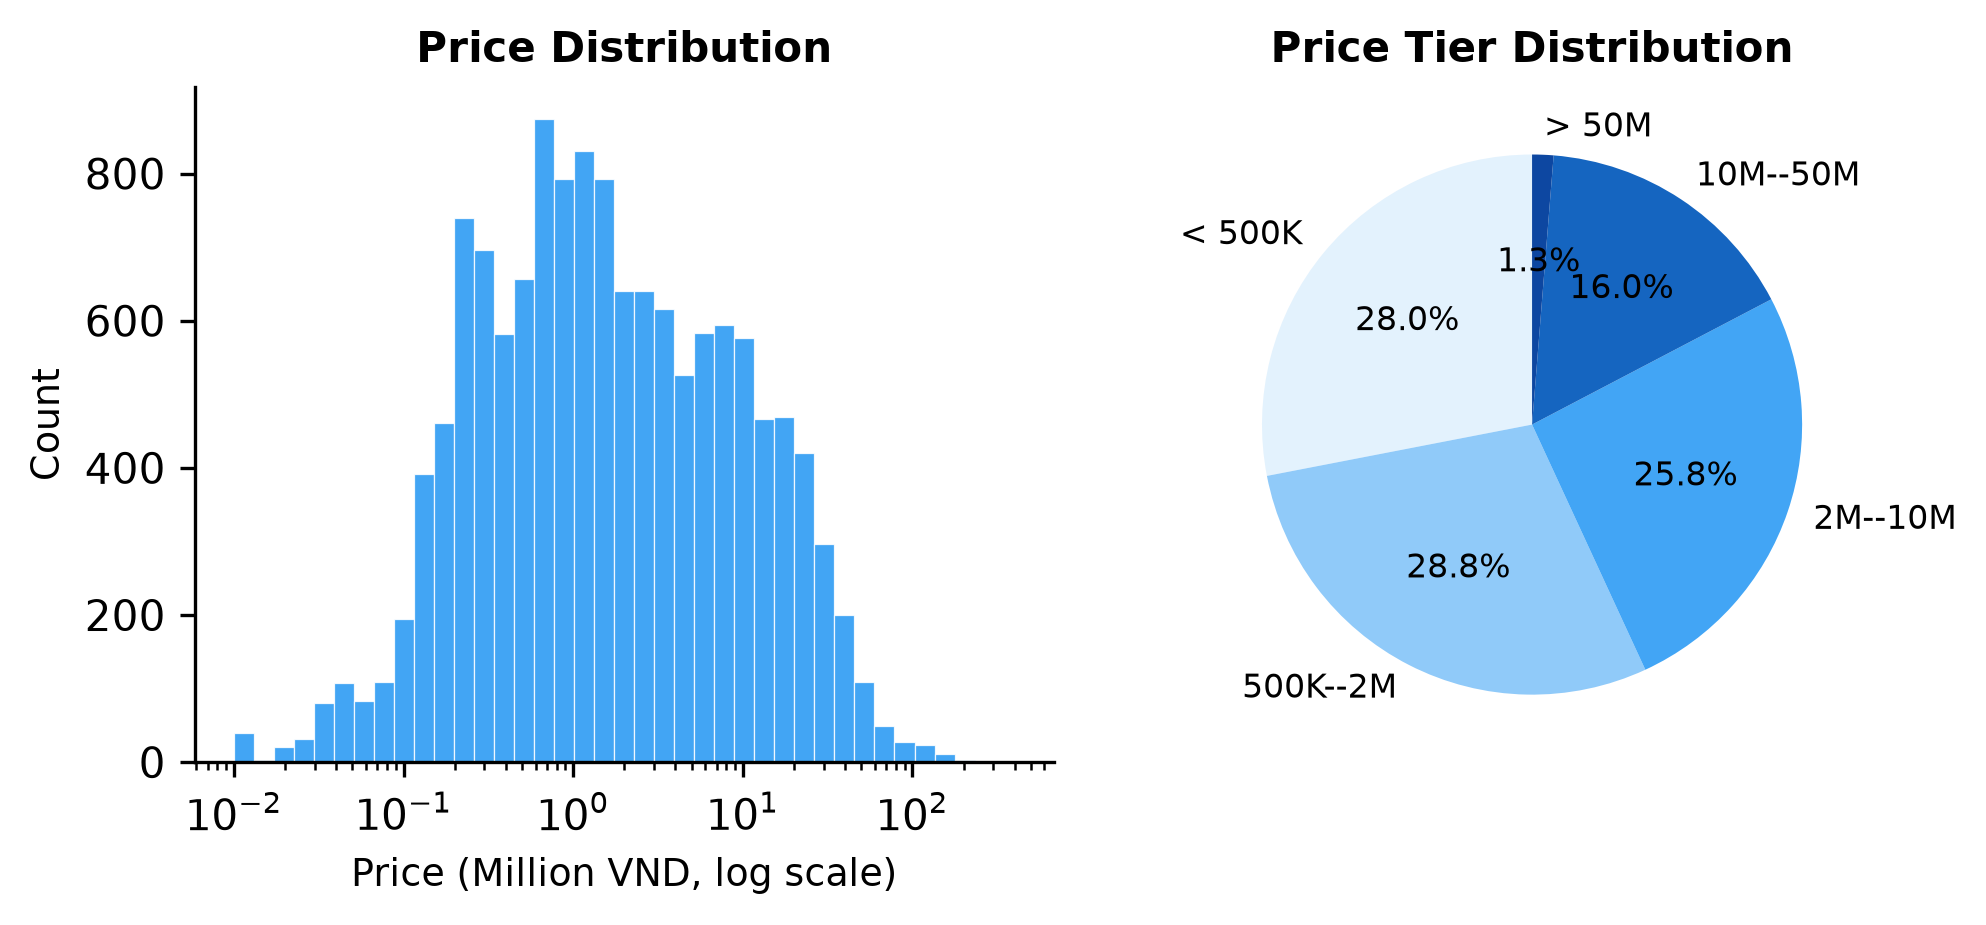
\includegraphics[width=\columnwidth]{figures/dataset_price_distribution.png}}
\caption{Price distribution detail. Left: log-scale histogram; right: price-tier segmentation showing 57\% of products in the 500K--10M~VND range.}
\label{fig_pricedist}
\end{figure}

\subsection{Conversational trajectory analysis}
Table~\ref{tab_chat} profiles 10 anonymized purchase-completion conversations recorded from the retailer's existing chatbot.

\begin{table}[htbp]
\caption{Chat Trajectory Statistics}
\begin{center}
\footnotesize
\begin{tabular}{|l|r|}
\hline
\textbf{Metric} & \textbf{Value} \\
\hline
Conversations & 10 \\
Total messages & 398 \\
Avg.\ messages / conversation & 39.8 \\
User messages & 133 \\
Assistant messages & 199 \\
Tool-call invocations & 56 \\
Distinct tools used & 7 \\
Conversations with purchase & 10 / 10 \\
\hline
\end{tabular}
\label{tab_chat}
\end{center}
\end{table}

Tool usage is dominated by order creation (22 calls, 39\%) and product search~(17, 30\%), followed by delivery-time queries~(11, 20\%). The remaining four tools---customer info check, product comparison, payment, and installment---together account for 11\%.

User messages exhibit Vietnamese informal patterns: abbreviated forms (\viet{dc}${\to}$\viet{được}, \viet{ko}${\to}$\viet{không}, \viet{sp}${\to}$\viet{sản phẩm}), mixed-case diacritics, and multi-product requests within a single turn. These patterns informed the abbreviation registry integrated into SalePilot's need extractor.

\subsection{Policy knowledge complexity}
The knowledge base ingests 7 policy documents (106 chunks after smart splitting). Warranty and return policies contain 6 product-group--specific fee schedules that vary by month since purchase. Delivery policies branch on distance, product type, order value, and geographic region. This structured complexity motivates the metadata-aware retrieval scorer described in Section~III.

\section{Evaluation Protocol}
\subsection{Benchmark and experimental boundary}
Fig.~\ref{fig2} summarizes the executable pipeline: every condition consumes the same sealed episodes and hash-pinned catalog, and every output artifact is hashed for independent reruns.

\begin{figure}[!t]
\centerline{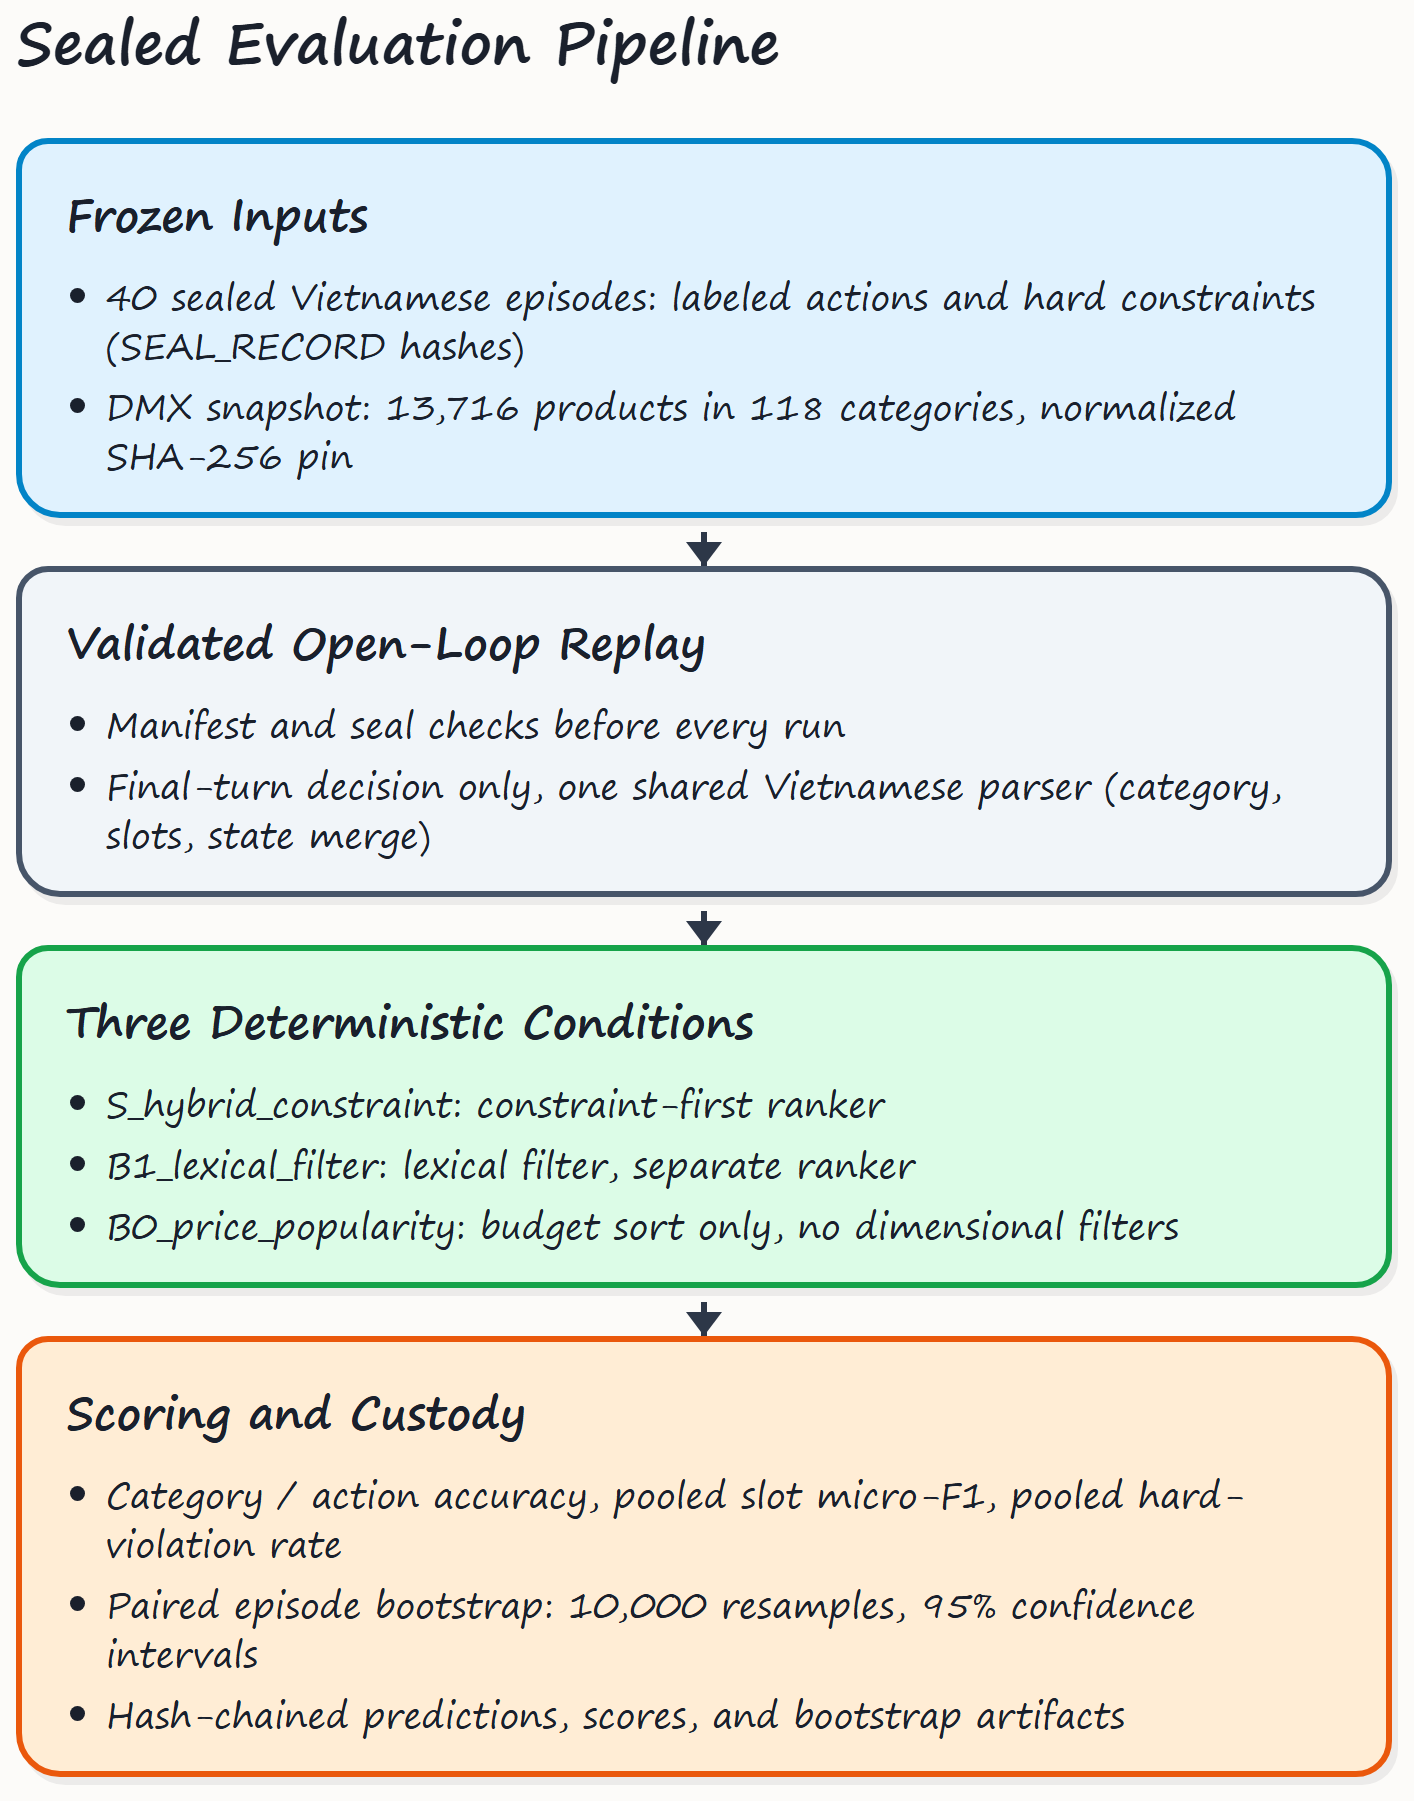
\includegraphics[width=0.92\columnwidth]{figures/evaluation_pipeline.png}}
\caption{Sealed evaluation pipeline. Identical frozen inputs and one shared parser isolate action policy and ranking as the only varying factors.}
\label{fig2}
\end{figure}

The sealed test set contains 40 developer-authored, single-turn Vietnamese episodes. It covers 11 non-null product categories plus FAQ and out-of-scope cases, including clarification, abstention, negation, and no-diacritics inputs.

The fixed evaluation snapshot contains 13{,}716 products in 118 categories (a strict subset of the full 13{,}754-product crawl described in Section~IV, filtered to records present at evaluation time). Its normalized SHA-256 is shown below, with one layout line break:

\begin{center}
\footnotesize\texttt{e2afdf38ed2df5599611e6f8285643f7}\\[-1pt]
\texttt{27e2c06c721b1a055b7baeea797df15c}
\end{center}

Turns are replayed open-loop. Only the prediction after the final user turn is scored. The Lead loop, specialist roles, databases, persistence, generated wording, frontend, and channel controls are not executed.

\subsection{Systems}
All three systems share category detection, slot extraction, and state merge. This isolates action and ranking differences but prevents the comparison from testing alternative Vietnamese parsers.

\texttt{S\_hybrid\_constraint} uses the production ranker with configured slot and preference terms. \texttt{B1\_lexical\_filter} uses lexical overlap, popularity, explicit filters, and a separate ranking implementation.

\texttt{B0\_price\_popularity} filters missing prices and over-budget items, then sorts by popularity and price. It does not apply the remaining dimensional or category-specific filters.

An optional LLM baseline is omitted from the primary comparison. Its checked-in provider pin, prediction bytes, catalog, and score artifacts do not form one consistent custody chain.

Fig.~\ref{fig_evalworkflow} shows the intended four-comparator design. B2\_llm\_single\_agent is depicted for completeness but is excluded from primary results due to an inconsistent provider custody chain (see Section~V-D for detail).

\begin{figure}[!t]
\centerline{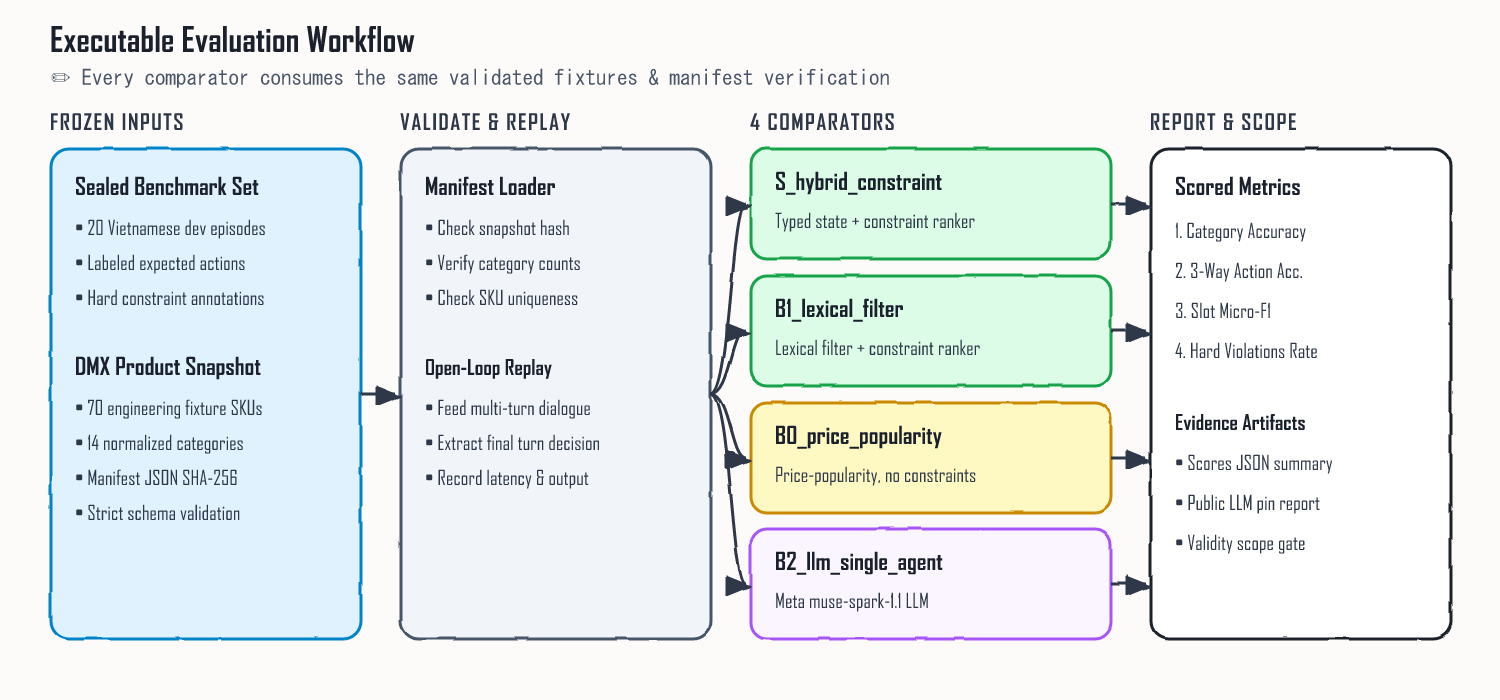
\includegraphics[width=\columnwidth]{figures/evaluation_workflow.png}}
\caption{Full four-comparator evaluation design. Each comparator consumes the same sealed benchmark and hash-pinned snapshot. B2 (LLM single-agent) is excluded from the primary analysis due to an inconsistent provider custody chain.}
\label{fig_evalworkflow}
\end{figure}

\subsection{Metrics and custody}
Category accuracy includes all 40 episodes, including null-category labels. Action accuracy covers the four classes emitted by these systems: recommend, clarify, FAQ, and abstain.

Slot micro-F1 pools true positives, false positives, and false negatives across structured need fields. It is not the mean of episode-level F1 values.

Hard-constraint violation rate pools product--constraint pairs over returned products. A check compares one returned product with one labeled hard constraint, applying that constraint's missing-data policy.

Prediction, score, and bootstrap files are hashed in a chain-of-custody record. The test file and catalog are also hash-pinned, although the record does not pin a code revision or conditions-file hash.

Frozen inputs and explicit configurations address documented reproducibility problems in recommender research~\cite{beel2016reproducibility}.

The artifact practice also mirrors parts of the NeurIPS reproducibility program, including code submission and checklists~\cite{pineau2021reproducibility}.

\section{Results and Evidence Boundary}
\subsection{Quantitative results}
Table~\ref{tab1} reports the three deterministic conditions on the same sealed split and evaluation snapshot.

\begin{table}[htbp]
\caption{Results on 40 Sealed Vietnamese Episodes and the 13{,}716-Product Evaluation Snapshot}
\begin{center}
\footnotesize
\setlength{\tabcolsep}{4pt}
\begin{tabular}{|l|c|c|c|c|c|}
\hline
\textbf{System}&\textbf{Cat.}&\textbf{Act.}&\textbf{Slot $\mu$F1}&\textbf{Hard Viol.}&\textbf{Chk}$^{\mathrm{a}}$ \\
\hline
S\_hybrid& 0.950& 0.850& 0.942& \textbf{0.000}& 99 \\
\hline
B1\_lexical& 0.950& 0.850& 0.942& \textbf{0.000}& 99 \\
\hline
B0\_popularity& 0.950& \textbf{0.925}& 0.942& 0.0855& 117 \\
\hline
\multicolumn{6}{l}{$^{\mathrm{a}}$Cat./Act.: category and action accuracy. Slot $\mu$F1: pooled slot} \\
\multicolumn{6}{l}{micro-F1. Hard Viol.: pooled violations per product--constraint} \\
\multicolumn{6}{l}{check. Chk: checks evaluated.}
\end{tabular}
\label{tab1}
\end{center}
\end{table}

All conditions obtain 0.950 category accuracy and 0.942 slot micro-F1 because they share the same parser. These ties do not show that the parser is optimal or that ranking has no effect.

B0 obtains higher action accuracy: 0.925 versus 0.850. Its simpler admission policy avoids some clarifications, but its returned lists produce 10 violations across 117 checks.

Those violations comprise six area checks, three budget checks, and one width check. B1 and S\_hybrid produce no observed violations across 99 checks each.

The exposure also differs: B0 faces 117 product--constraint checks versus 99 because B1 and S\_hybrid more often clarify instead of recommending, so violation removal combines filtering with a more conservative action policy.

Episode-resample bootstrap intervals (10{,}000 resamples) estimate the pooled table metrics directly. All conditions are evaluated on identical resamples, so violation-rate differences are paired.

B0's pooled violation rate is 0.0855 with 95\% CI $[0.010, 0.167]$. The paired B0 minus S\_hybrid difference is 0.0855 with the same interval, excluding zero; the B0 minus B1 difference is identical.

B1 and S\_hybrid show zero violations in all resamples, so their percentile intervals are degenerate at zero. Under a rule-of-three reading that treats checks as independent, 0 of 99 bounds the rate below about 0.03~\cite{hanley1983zero}.

B1 and S\_hybrid tie on every reported aggregate. Their top-three SKU sequences differ on 28 episodes, but the benchmark has no item-relevance labels. It cannot establish which ranking is more useful.

The evidence supports one statistically grounded claim: explicit constraint filtering eliminates the observed violations that the price--popularity policy admits. It does not show superiority of S\_hybrid over B1 or generalization.

\subsection{Decision-evidence boundary}
A reviewer with access to the repository can re-run the deterministic evaluator against the pinned snapshot without invoking an LLM or network service. The sealed predictions, scores, bootstrap artifacts, and chain-of-custody record are in the \texttt{experiments/} directory. The anonymous supplement at submission time contains a legacy 8-scenario synthetic evaluation that does not reproduce the results in this paper.

The same implementation constructs the status fields and recommendations. The payload is therefore inspectable evidence, not independent certification. Frontend rendering and human comprehension were not evaluated.

\subsection{Deployment evidence}
At the recorded public check on 25 July 2026, the frontend returned HTTP 200 in 426.96 ms. The backend health endpoint returned HTTP 502 in 138.2 ms.

Chat, product, and fallback probes were skipped after the failed health check. The evidence supports public frontend reachability and local prototype configuration, not a healthy public end-to-end deployment.

\subsection{Threats to validity}
The benchmark is developer-authored, not an independently sampled or dual-annotated field corpus. Rule, scenario, and evaluator co-development can overfit the 40 episodes.

Open-loop final-turn replay does not test interactive question policy or user adaptation. Shared extraction makes the comparison chiefly about action and filtering, not end-to-end CRS quality.

The full catalog covers 119 categories (Section~IV), but the evaluation snapshot pins 118 and the test set has 11 labeled product categories. No relevance judgments support ranking metrics, and the inconsistent optional LLM artifacts prevent a like-for-like B2 comparison.

Reported intervals resample whole episodes and recompute pooled metrics~\cite{efron1979bootstrap}. They capture episode-sampling variability only, not authorship bias or the dependence of multiple checks inside one episode.

The custody record pins data and output hashes but not the code revision or conditions hash. Runtime identity, privacy, tool safety, orchestration, and public availability also remain outside the experiment.

Our planned external study targets at least 80 Vietnamese conversations, two independent annotators, and graded relevance labels. This sample target is project-specific and requires a separate precision analysis.

We will choose agreement coefficients according to label scale and assumptions~\cite{artstein2008agreement}. Uncertainty analysis will resample whole conversations and specify the bootstrap interval~\cite{efron1979bootstrap}.

User-facing constructs will be declared from CRS-Que before collection~\cite{jin2024crsque}. Until that study is complete, we make no claim about usefulness, trust, fluency, or conversion.

\section{Conclusion}
SalePilot is a Vietnamese retail prototype that separates deterministic recommendation from optional LLM orchestration and emits inspectable evidence for its deterministic routes.

The dataset analysis (Section~IV) reveals a severely imbalanced catalog---the top category holds 22.8\% of products while core appliance categories hold under 2\%---with a four-order-of-magnitude price range and sparse coverage on 4 of 29 fields. The 10 purchase conversations show that order creation and product search dominate tool usage (69\% of calls), and user messages exhibit Vietnamese informal patterns that standard tokenizers do not handle.

On one sealed, developer-authored 40-episode benchmark, B1 and S\_hybrid show no observed violations in 99 checks, while B0 shows 10 in 117; the paired difference of 0.0855 (95\% CI 0.010--0.167) excludes zero.

These results support explicit fail-closed filtering within the evaluated setup. They do not establish ranking utility over B1, end-to-end agent quality, field effectiveness, or healthy public deployment.

The artifact hashes, evidence dictionary, and candid scope boundary provide a basis for independent reruns. External annotation, relevance judgments, and an auditable LLM baseline remain future gates.

\section*{Acknowledgment}
AI coding assistants supported language drafting, bibliographic collection, diagram review, and consistency checks against source code and evaluator artifacts. They did not generate the reported measurements.

The authors remain responsible for verifying the manuscript, sources, measurements, and disclosure before submission.

\bibliographystyle{IEEEtran}
% Balance the final-page reference columns without changing IEEE margins.
\IEEEtriggeratref{19}
\bibliography{ref}

\end{document}
